\pagestyle{plain}
\documentclass[a4paper]{jarticle}
\usepackage{geometry}
\usepackage{amsmath}
\usepackage[dvips]{graphicx}
\usepackage{multicol}
\usepackage{here}
\geometry{left=25mm,right=25mm,top=30mm,bottom=30mm}


\title{ハイブリッドロケットの飛翔シミュレーション}
\author{兼松 翼}

\begin{document}
\maketitle

\begin{abstract}
  本資料はハイブリッドロケットの飛翔経路を計算するための,6自由度の運動方程式を用いたシミュレーション手法についてまとめたものである.
  また,巻末に各記号の説明を載せたので同時に参照されたい.また, 簡単なフローチャートも記載した.
\end{abstract}


%------------------------------------
%-   座標系                          -
%------------------------------------
\section{座標系}

本プログラムでは機体座標系と地上座標系を用いる.
機体座標系\(x_B,y_B,z_B\)は,機体重心を原点とし,機軸前向きを\(x_B\)軸,右向きを\(y_B\),下向きを\(z_B\)軸とする.
また,角速度およびモーメントは,軸の正方向をみて,時計回りを正とする.オイラ角に関しても同様である.

地上座標系は,慣習とは異なり鉛直上向きを\(z_E\)の正方向とした.本プログラムでは風の影響を考慮するため\(x_E\)と\(y_E\)はそれぞれ,磁東,磁北とした.

\begin{figure}[h]
  \begin{tabular}{cc}
    \begin{minipage}[t]{0.45\hsize}
      \centering
       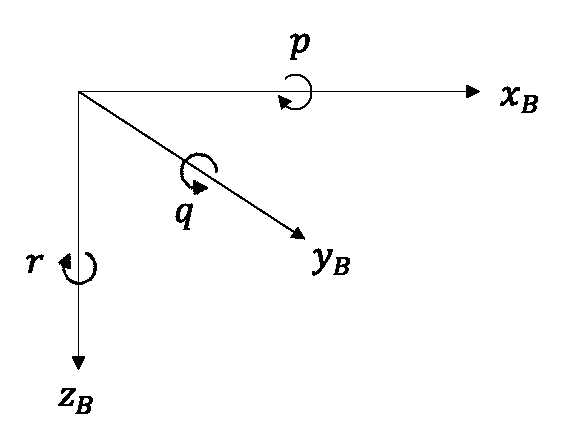
\includegraphics[keepaspectratio, scale=0.5]{./figure1.eps}
       \caption{機体座標系}
       \label{fig:one}
      \end{minipage} &

    \begin{minipage}[t]{0.45\hsize}
      \centering
      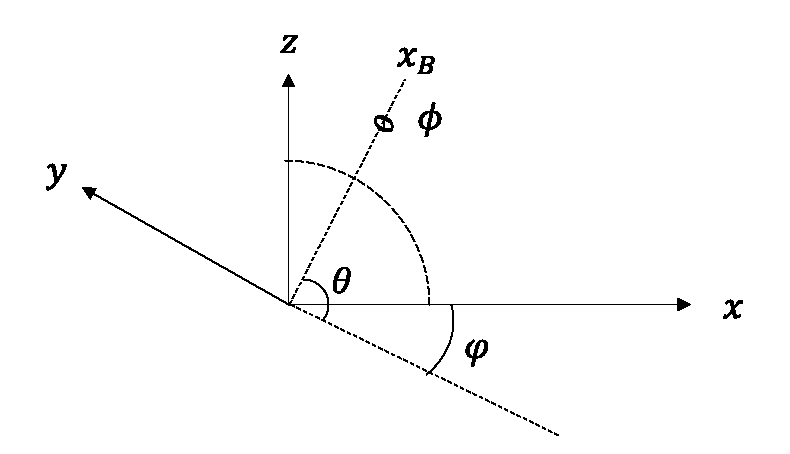
\includegraphics[keepaspectratio, scale=0.5]{./figure2.eps}
      \caption{機体座標系と地上座標系}
      \label{fig:two}
    \end{minipage}
  \end{tabular}
\end{figure}

迎え角および横滑り角については次式のように定義する.
\begin{equation}
  \alpha = tan^{-1} \frac{V_{azB}}{V_{axB}},  \beta = sin^{-1} \frac{V_{ayB}}{V_{aB}}
\end{equation}

\section{風速モデル}
風による機体への影響を求めるためには対気速度を求める必要があるが,次式により求めることができる.
\begin{equation}
  \begin{cases}
    V_{ax} = V_{xB} - V_{wx} \\
    V_{ay} = V_{yB} - V_{wy} \\
    V_{az} = V_{zB} - V_{wz}
  \end{cases}
\end{equation}
\begin{equation}
  V_{a} = \sqrt{V_{ax}^2+V_{ay}^2+V_{az}^2}
\end{equation}

\(V_{wx}\),\(V_{wy}\),\(V_{wz}\)は対地風速であるが,風の流れは地面の影響を受けており,
高度が上がるごとに風速は強くなるので,経験則的に求められたべき分布を用いて計算する必要がある.

\begin{equation}
  \begin{cases}
    V_{wx} = V_w cos (\frac{Vw_{angle} \pi}{180} )(\frac{Z}{H_w})^\frac{1}{W_h} \\
    V_{wy} = V_w sin (\frac{Vw_{angle} \pi}{180} )(\frac{Z}{H_w})^\frac{1}{W_h} \\
    V_{wz} = 0
  \end{cases}
\end{equation}

%-----------------------------------
%-    運動方程式                     -
%------------------------------------
\section{機体に加わる外力}

本プログラムにおいて推力Tは,燃焼実験における実測値を用い,ミスアライメントはないものとしたため単に
\begin{equation}
  T_x = T, T_y = T_z = 0
\end{equation}
とした.

\(S\)を機体断面積, \(\rho\)を空気密度, \(V_{\alpha}\)を対気速度, \(C_d\),\(C_N\),\(C_N\)をそれぞれ抗力係数,垂直力係数とすると,空気力による力は次式で表される.
\begin{equation}
  \begin{cases}
    D = (1/2)S \rho V_{\alpha}^2 C_D \\
    Y = (1/2)S \rho V_{\alpha}^2 C_Y \beta \\
    N = (1/2)S \rho V_{\alpha}^2 C_N \alpha
  \end{cases}
\end{equation}

\(G_{xB}\), \(G_{yB}\), \(G_{zB}\)は機体座標系における重力加速度であり, \(g\)を重力加速度とすると次式により表される.
\begin{equation}
  \left(
    \begin{array}{ccc}
      G_x \\
      G_y \\
      G_z
    \end{array}
  \right) = A_{\overrightarrow{EB}}
  \left(
    \begin{array}{ccc}
      0 \\
      0 \\
      -g
    \end{array}
  \right)
\end{equation}

機体に加わるモーメントは次式のように求められる.

\begin{eqnarray}
  \begin{cases}
    M_p = M_{FM} + \frac{1}{4} \rho S V_a d^2 C_{lp} p \\%+ M_{jp} \\
    M_q = -(l_{Cp}-l_{CG})N + \frac{1}{4} \rho S V_a l^2 C_{mq} q \\% + M_{Jq} \\
    M_r = -(l_{Cp}-l_{CG})Y + \frac{1}{4} \rho S V_a l^2 C_{nr} r \\% + M_{Jr}
  \end{cases}
\end{eqnarray}

上式の第1項は空気力による加速側のモーメント,第2項は空気力による減衰モーメントである.
なお, \(M_{FM}\)はフィンのミスアライメントであるが製作したプログラムでは\(M_{FM} = 0\)としている.

\section{運動方程式}
ロケットの飛翔経路は, 地上座標系における機体速度を積分することによって得られる.微分方程式で以下のように示される.  
\begin{equation}
\left(
  \begin{array}{ccc}
    \dot X \\
    \dot Y \\
    \dot Z 
  \end{array}
\right)=
\left(
  \begin{array}{ccc}
    V_{xE} \\
    V_{yE} \\
    V_{zE}  
  \end{array}
\right)
\end{equation}

上式の右辺は機体座標系における速度に座標変換行列$A_{\overrightarrow{BE}}$を掛けることによって求めることができる.
しかし,後述するが座標変換行列のみでの計算は特異点や計算速度などの問題があるので,本来ならばクォータニオンを用いるのが良い.

\begin{equation}
\left(
  \begin{array}{ccc}
    V_{xE} \\
    V_{yE} \\
    V_{zE}  
  \end{array}
\right)=A_{ \overrightarrow{BE} }
\left(
  \begin{array}{ccc}
    V_{xB} \\
    V_{yB} \\
    V_{zB}  
  \end{array}
\right)
\end{equation}


\begin{equation}
A_{ \overrightarrow{BE} }=
\left(
  \begin{array}{ccc}
    cos \theta cos \psi & sin \phi sin \theta cos \psi - cos \phi sin \psi & cos \phi sin \theta cos \psi + sin \phi sin \psi \\
    cos \theta sin \psi & sin \phi sin \theta sin \psi + cos \phi cos \psi & cos \phi sin \theta sin \psi - sin \phi cos \psi \\
    -sin \theta & sin \phi cos \theta &cos \phi cos \theta
  \end{array}
\right)
\end{equation}

機体座標系における速度は,機体座標系における加速度を積分することによって得られ,その加速度は次式で表される. 
\begin{eqnarray}
    \begin{cases}
      \dot V_{xB} = (T_x-D)/m + (rV_{yB}-qV_{zB})+G_x \\
      \dot V_{yB} = (T_y+Y)/m + (p_zV_B-rV_{xB})+G_y \\
      \dot V_{zB} = (T_z-N)/m + (qV_{xB}-pV_{xB})+G_z
    \end{cases}
\end{eqnarray}  

ここで第2項はコリオリの力によるものである.
また, 上式で用いたモーメントと慣性モーメント,角速度を用いて角速度の微分系を表すと次のようになる.

\begin{eqnarray}
  \begin{cases}
    \dot p = {(I_y-I_z)qr+M_p}/I_x \\
    \dot q = {(I_z-I_x)rp+M_q}/I_y \\
    \dot r = {(I_x-I_y)pq+M_r}/I_z 
  \end{cases}
\end{eqnarray}

第1目はジャイロ効果によるものである.
オイラー角は次式を積分することによって求める.

\begin{eqnarray}
  \begin{cases} 
    \dot \phi = p + tan \theta (q sin \phi + r cos \phi) \\
    \dot \theta = q cos \phi - r sin \phi \\
    \dot \psi = (q sin \phi + r cos \phi)sec \theta
  \end{cases}
\end{eqnarray}

ただし, \( \theta = 90[deg]\)付近において\(tan \theta \)の値が異常に大きくなって積分ができなくなるので,次式に変えて計算する.
\begin{eqnarray}
  \begin{cases}
    \dot \phi = p + sin \theta ・ \frac{q sin \phi +r cos \phi}{cos \theta} \\
    \dot \theta = q cos \phi - r sin \phi - r sin \phi \\
    \dot \psi = \frac{q sin \theta + r cos \phi}{cos \theta}
  \end{cases}
\end{eqnarray}
%-----------------------------------
%-     質量計算                     -
%-----------------------------------
\section{質量計算}

燃焼中,ロケットは推進剤を高速で噴射することにより,運動量推力を発生させている.
そのため, シミュレーション上でもそれに伴う質量変化を考慮する必要がある.酸化剤質量流量と燃料質量流量が既知の場合には,
それらを積分することによって\(m_{ox}\)と\(m_f\)を得られるので次式を用いて容易に求めることができる.

\begin{eqnarray}
  m_p = m_{ox} + m_f \\
  m = m_p + m_s
\end{eqnarray}


%-----------------------------------
%-     重心位置                     -
%-----------------------------------
\section{重心位置}

また,重心位置は次式によって求めることができる. ただし, 燃焼系部(主にモータとタンク)の重心位置については, ノーズ先端ではなくエンドカバーからの位置としている.

\begin{eqnarray}
  l_{cgox} = l_{cgox0} - \frac{1}{2}(1 - \frac{m_{ox}}{m_{ox0}}) * l_{tank} \\
  l_{cgp} = \frac{m_f * l_{cgf} + m_{ox} * l_{cgox}}{m_f + m_{ox}} \\
  lcg = \frac{m_p * l_{cgp} + m_s * l_{cgs}}{m}
\end{eqnarray}

\begin{figure}[htbp]
  \centering
  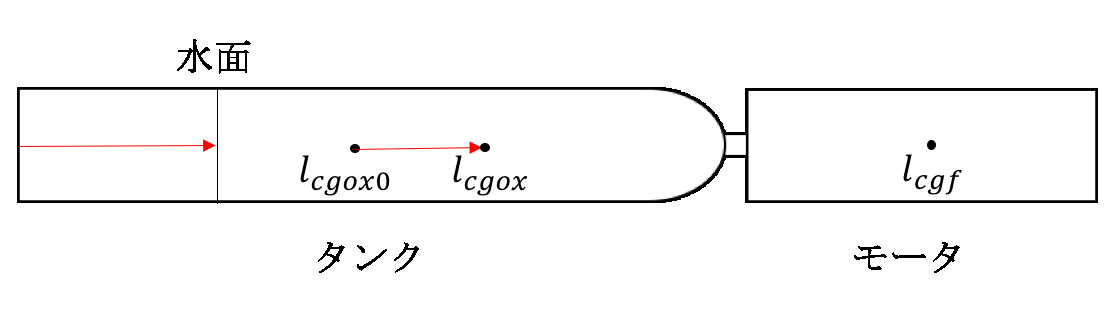
\includegraphics[width=100mm]{figure3.eps}
  \caption{燃焼部簡略図}
\end{figure}
%------------------------------------
%-    計算例                         -
%------------------------------------
\section{計算結果}
実際にシミュレーションを行なった結果を示す.以下の諸元はH-45のものである.

\begin{table}[H]
  \centering
  \begin{tabular}{|l|l|r|r|} \hline
    記号 & 要素 & 値 & 単位 \\ \hline
    $P_a$ & 大気圧 & 100.8 & kPa \\ \hline
    $T$ & 気温 & 25.0 & deg \\ \hline
    $\rho$ & 大気密度 & 1.18 & $kg/m^3$ \\ \hline
    $g$ & 重力加速度 & 9.80 & $m/s^2$ \\ \hline
    $H_w$ & 風速測定点 & 5.00 & m \\ \hline
    $W_h$ & 高度分布係数 & 4.5 & \\ \hline
    $\theta$ & 射角 & -84.0 & deg \\ \hline
    $\psi$ & 方位角 & 235.0 & deg \\ \hline
    $l_L$ & ランチャ長 & 5.0 & m \\ \hline
  \end{tabular}
  \caption{環境条件}
\end{table}

\begin{table}[H]
  \centering
  \begin{tabular}{|l|l|r|r|} \hline
    記号 & 要素 & 値 & 単位 \\ \hline
    $L$ & 全長 & 1.627 & m \\ \hline
    $S$ & 機体直径 & 0.154 & m \\ \hline
    $m_S$ & 機体空虚質量 & 7.781 & kg \\ \hline
    $l_{CGS}$ & 機体空虚重心位置 & 0.897 & m \\ \hline
    $l_{CGox}$ & 酸化剤重心位置 & 0.441 & m \\ \hline
    $l_{CGf}$ & 燃料重心位置 & 0.118 & m \\ \hline
    $l_{tank}$ & タンク長さ & 0.3 & m \\ \hline
    $l_{pitch}$ & 慣性モーメント(Pitch・Yaw) & 1.814 & $kgm^2$ \\ \hline
    $l_{roll}$ & 慣性モーメント(roll) & 0.022 & $kgm^2$ \\ \hline
    $l_{cp}$ & 圧力中心 & 1.132 & m \\ \hline
    $C_{lp}$ & 減衰モーメント係数 & -0.13 &  \\ \hline
    $C_{mq}$ & 減衰モーメント係数 & -2.21 & \\ \hline
    $C_D$ & 抗力係数 & 0.55 & \\ \hline
    $C_{N}$ & 法線力係数 & 7.04 & \\ \hline 
    $C_DS$ & パラシュート抗力特性 & 0.675 & $m^2$ \\ \hline
    $freq$ & サンプリングレート & 3000 & Hz \\ \hline
    $m_{ox}$ & 酸化剤質量 & 0.389 & kg \\ \hline
    $m_fa$ & 全燃料質量 & 0.176 & kg \\ \hline
    $m_fb$ & 燃焼後燃料質量 & 0.145 & kg \\ \hline
    $\dot m_{ox}$ & 酸化剤質量流量 & 0.238 & kg/s \\ \hline
    $\dot m_f$ & 燃料質量流量 & 0.037 & kg/s \\ \hline
  \end{tabular}
  \caption{機体諸元}
\end{table}

\newpage

\begin{figure}[H]
  \begin{tabular}{cc}
    \centering
    \begin{minipage}{0.45\hsize}
      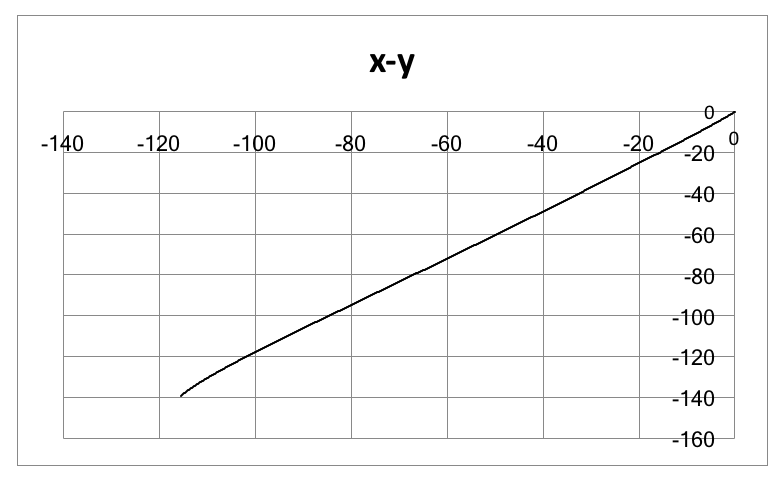
\includegraphics[scale=0.55]{./x-y.eps}
      \caption{2次元飛翔経路}
    \end{minipage} &
    \begin{minipage}{0.45\hsize}
       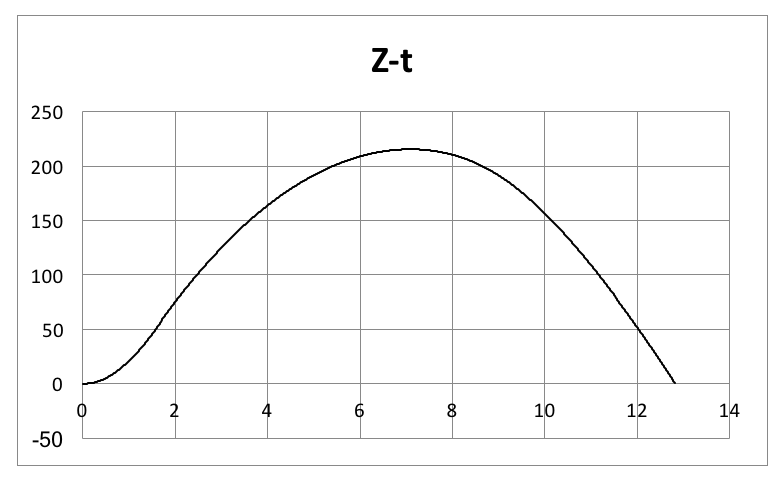
\includegraphics[scale=0.55]{./Z.eps}
       \caption{高度}
      \end{minipage}
  \end{tabular}
\end{figure}

\begin{figure}[H]
  \begin{tabular}{cc}
    \centering
    \begin{minipage}{0.45\hsize}
      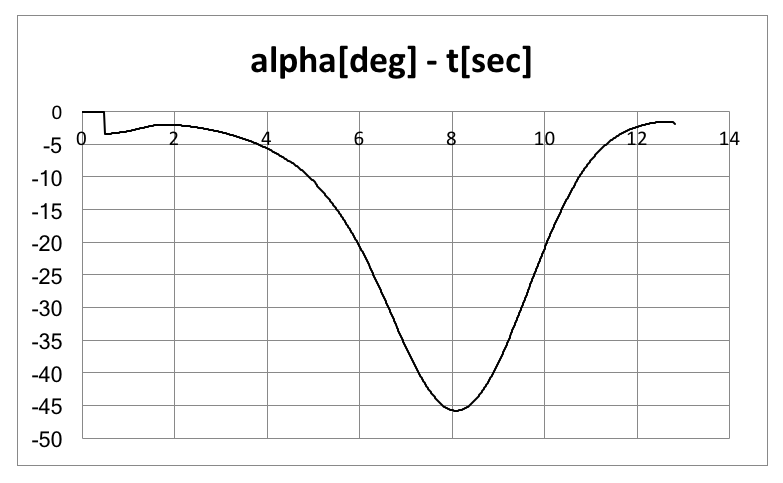
\includegraphics[scale=0.55]{./alpha.eps}
      \caption{迎え角}
    \end{minipage} &
    \begin{minipage}{0.45\hsize}
       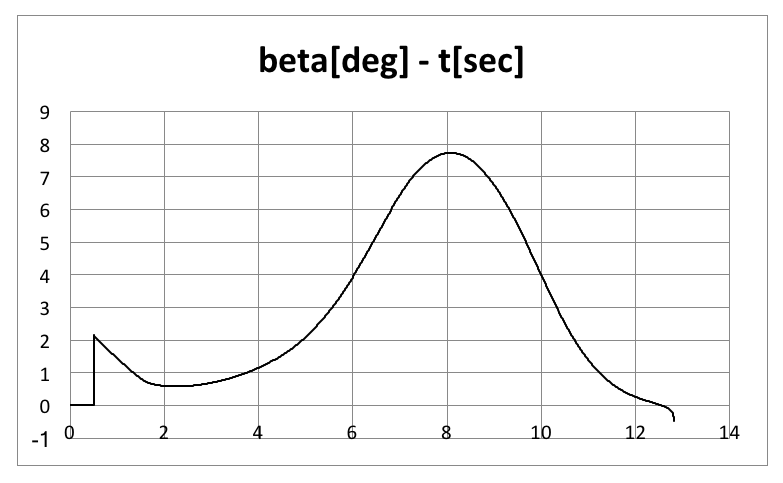
\includegraphics[scale=0.55]{./beta.eps}
       \caption{横滑り角}
      \end{minipage}
  \end{tabular}
\end{figure}

\begin{figure}[H]
  \begin{tabular}{cc}
    \centering
    \begin{minipage}{0.45\hsize}
      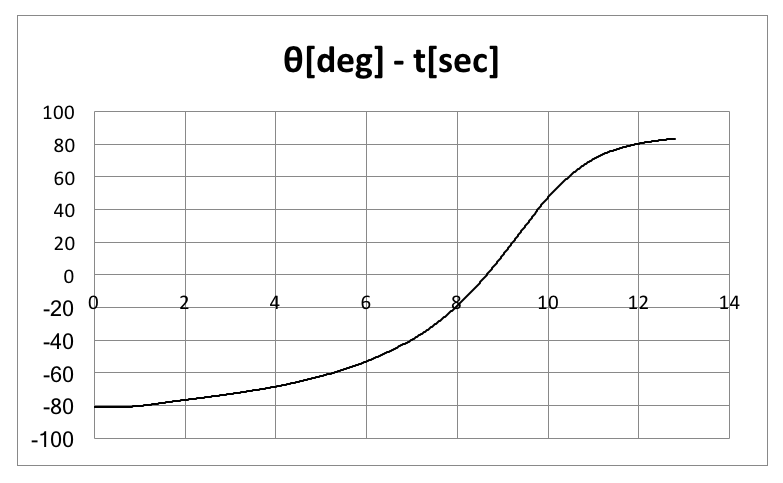
\includegraphics[scale=0.55]{./theta.eps}
      \caption{t-theta}
    \end{minipage} &
    \begin{minipage}{0.45\hsize}
       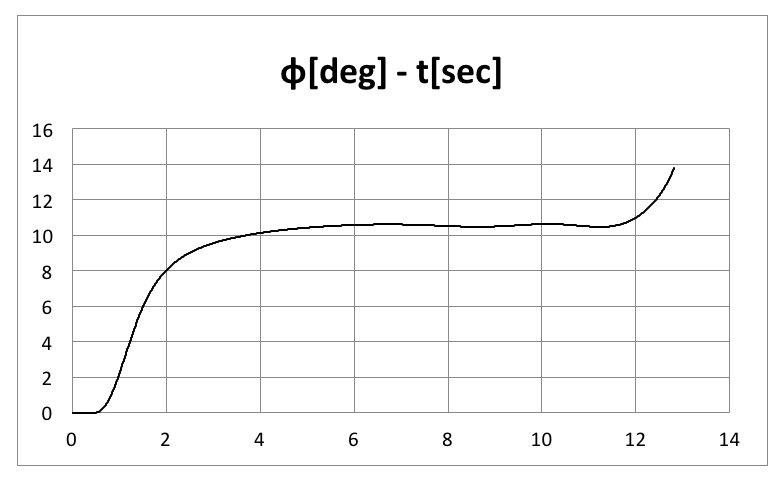
\includegraphics[scale=0.55]{./phi.eps}
       \caption{t-phi}
      \end{minipage}
  \end{tabular}
\end{figure}

\begin{figure}[H]
  \begin{tabular}{c}
    \centering
    \begin{minipage}{0.45\hsize}
      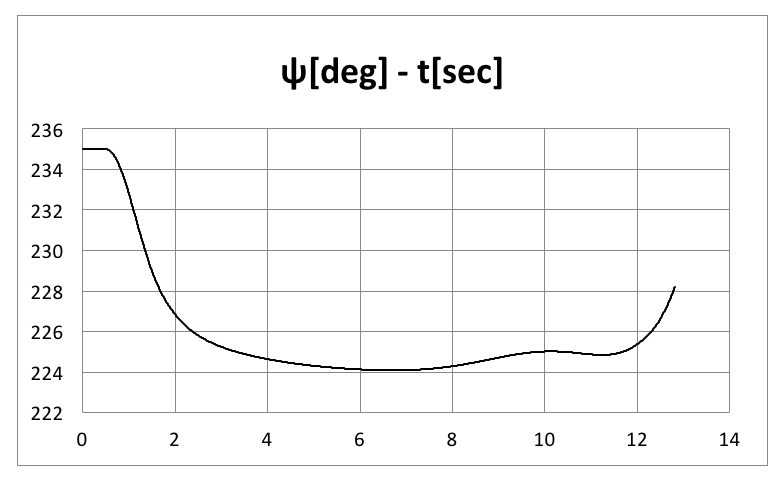
\includegraphics[scale=0.55]{./psi.eps}
      \caption{t-psi}
    \end{minipage} 
  \end{tabular}
\end{figure}

\begin{figure}[H]
  \begin{tabular}{cc}
    \centering
    \begin{minipage}{0.45\hsize}
       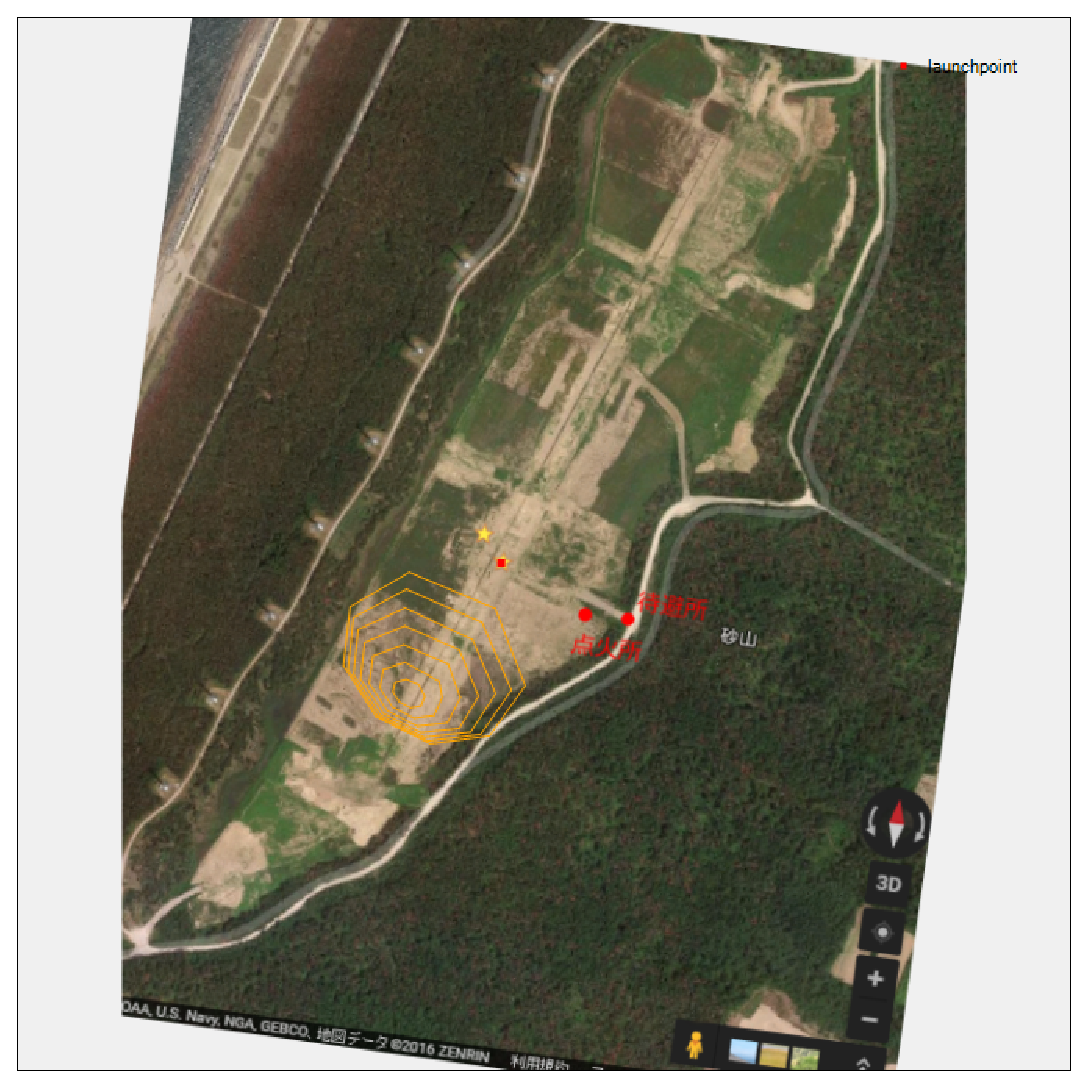
\includegraphics[scale=0.35]{./LandingPlotHard.eps}
       \caption{弾道落下分散}
      \end{minipage} &
    \begin{minipage}{0.45\hsize}
      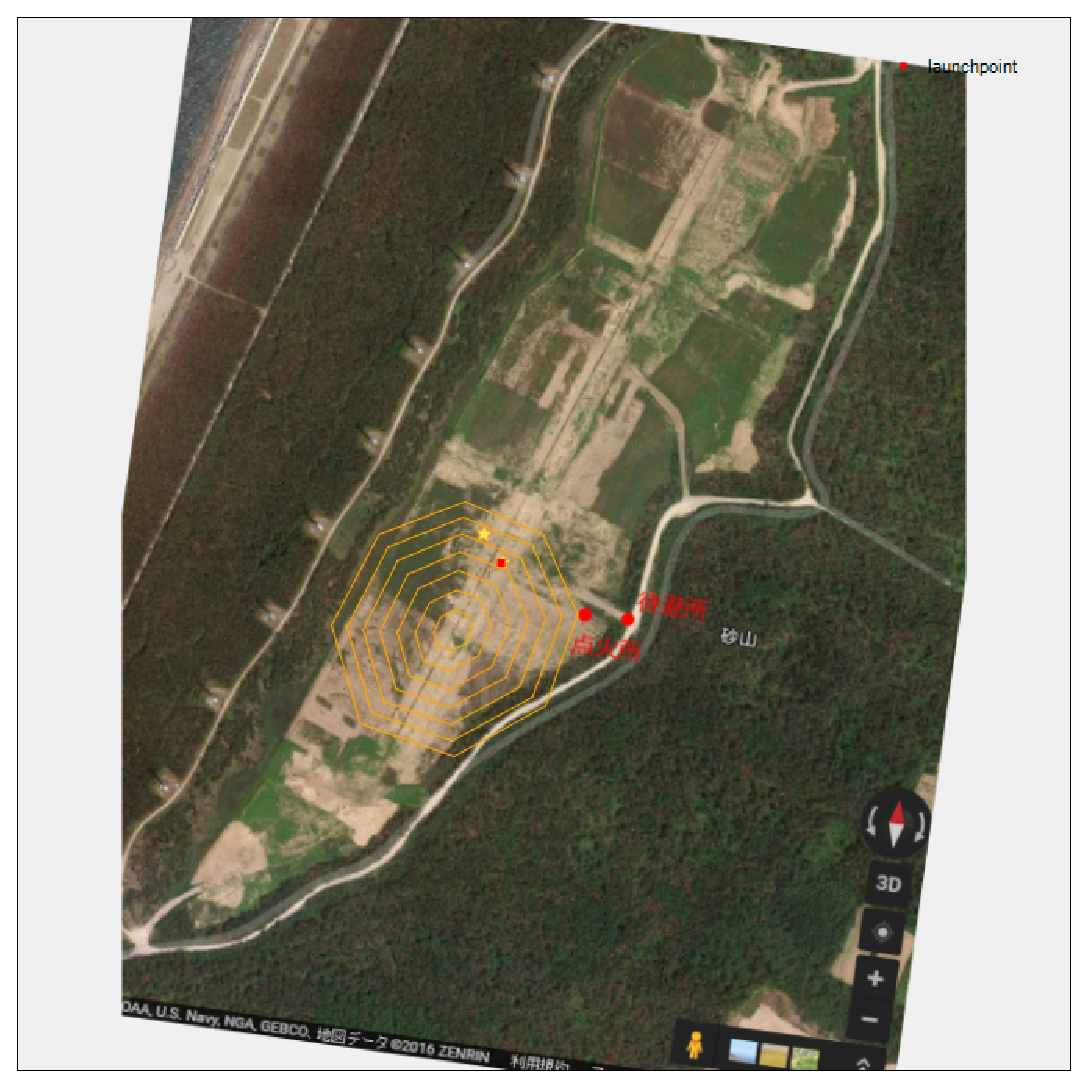
\includegraphics[scale=0.35]{./LandingPlotSoft.eps}
      \caption{減速落下分散}
    \end{minipage}
  \end{tabular}
\end{figure}

\appendix
%------------------------------------
%-   記号                            -
%------------------------------------
\newpage
\section{付録:記号}

\begin{multicols}{2}
  \begin{description}
    \item[$\alpha$] 迎え角[rad]
    \item[$\beta$] 横滑り角[rad]
    \item[$V_{a}, V_{ax}, V_{ay}, V_{az}$] 機体座標系における対気速度[m/s]
    \item[$V_{xB}, V_{yB}, V_{zB}$] 機体座標系における対地速度[m/s]
    \item[$V_{w}, V_{wx}, V_{wy}, V_{wz}$] 地上座標系における風速[m/s]
    \item[$V_{xE}, V_{yE}, V_{zE}$] 地上座標系における対地速度[m/s]
    \item[$W_h$] 高度分布係数
    \item[$H_w$] 風速測定点[m]
    \item[$X,Y,Z$] 変位[m]
    \item[$A_{ \overrightarrow{BE}},A_{\overrightarrow{EB}}$] 座標変換行列
    \item[$T,T_{x},T_{y},T_{z}$] 推力[N]
    \item[$D$] 抗力[N]
    \item[$Y,N$] 垂直力[N]
    \item[$S$] 機体断面積[$m^2$]
    \item[$\rho$] 大気密度[$kg/m^3$]
    \item[$C_d$] 抗力係数
    \item[$C_Y,C_N$] 垂直力係数
    \item[$G_x,G_y,G_z$] 機体座標系における重力[N]
    \item[$g$] 重力加速度[$m/s^2$]
    \item[$\theta$] 縦揺れ角[rad]
    \item[$\phi$] 横揺れ角[rad]
    \item[$\psi$] 偏揺れ角[rad]
    \item[$p,q,r$] 機体座標系における角速度[rad/s]
    \item[$m$] 全機質量[kg]
    \item[$m_p$] 推進剤質量[kg]
    \item[$m_{ox}$] 酸化剤質量[kg]
    \item[$m_f$] 燃料質量[kg]
    \item[$m_s$] 空虚機体質量[kg]
    \item[$l$] 機体全長[m]
    \item[$l_{tank}$] タンク長さ[m]
    \item[$M_p,M_q,M_r$] モーメント[Nm]
    \item[$M_{FM}$]フィンミスアライメントによるモーメント[Nm]
    \item[$M_{Jp},M_{Jq},M_{Jr}$] ジェットダンピングモーメント[Nm]
    \item[$C_{lp},C_{mq},C_{nr}$] 減衰モーメント係数
    \item[$I_x,I_y,I_z$] 全機の慣性モーメント[Nm]
    \item[$l_{cgox}$] 酸化剤重心位置(エンドカバーからの位置)[m]
    \item[$l_{cgf}$] 燃料重心位置(エンドカバーからの位置)[m]
    \item[$l_{cgp}$] 推進剤重心位置(エンドカバーからの位置)[m]
    \item[$l_{cgs}$] 空虚重心位置[m]
    \item[$l_{cg}$] 全機重心位置[m]
    \item[$Vw_{angle}$] 風向
  \end{description}
\end{multicols}

%------------------------------------
%-    フローチャート                  -
%------------------------------------
\section{付録:フローチャート}
\begin{figure}[H]
  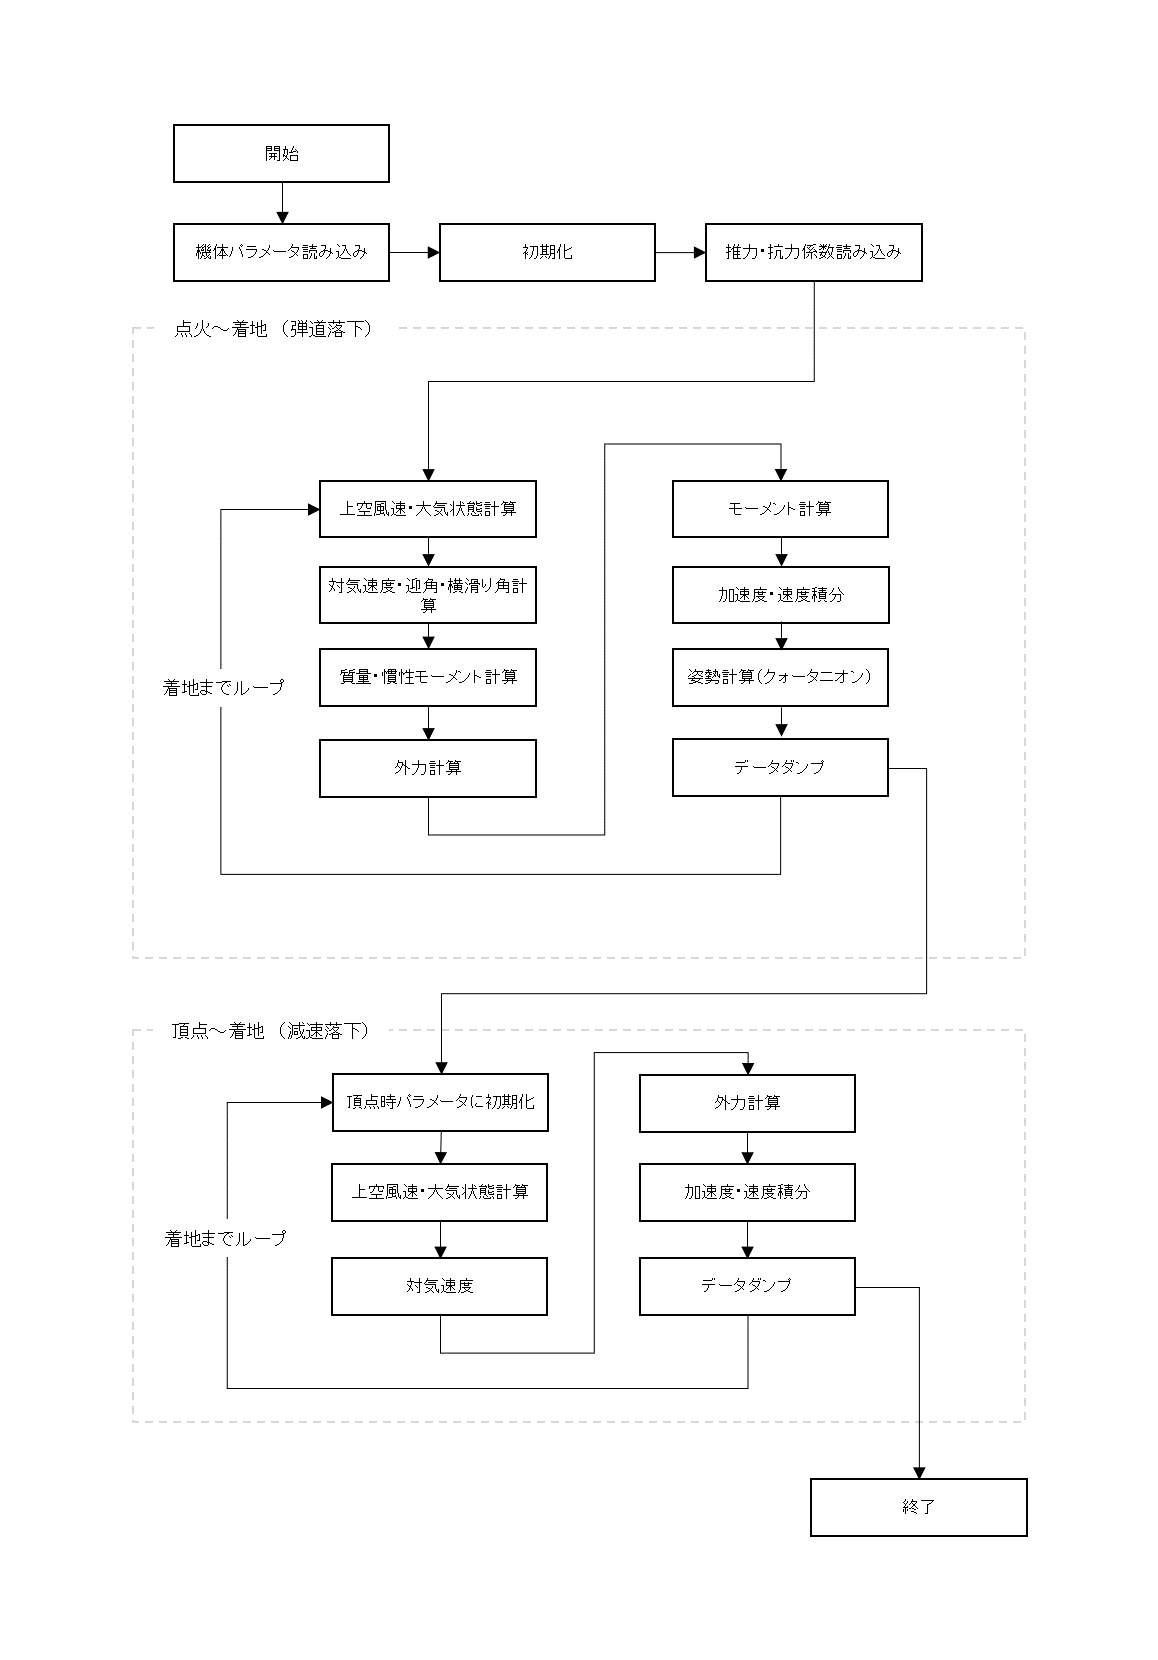
\includegraphics[scale=0.8]{./flowchart.eps}
\end{figure}

%------------------------------------
%-    参考文献                       -
%------------------------------------
\begin{thebibliography}{9}
  \bibitem{SPIN} 航空宇宙技術研究資料 TM-145 スピンを伴うロケットの運動を計算するプログラム
  \bibitem{QUATERNION} 航空宇宙技術研究資料 TM-636 クォータニオンとオイラー角によるキネマティック表現の比較
\end{thebibliography}



\end{document}

